
% ════════════════════════════════════════
% 模型检验与分析（06.模型检验.tex）
% ════════════════════════════════════════
\section{模型检验与分析}

为验证本文构建的模型的有效性和稳健性，进行以下检验。本文模型为线性规划优化模型，其最优性由求解器严格保证\cite{boyd2004}，因此检验重点在于约束满足程度、能量守恒精度与参数灵敏度。

\subsection{误差分析}

对问题一的最优解逐项核验其约束满足情况与能量守恒精度，结果如表\ref{tab:error}所示。

\begin{longtable}{>{\centering\arraybackslash}p{0.30\textwidth}>{\centering\arraybackslash}p{0.26\textwidth}>{\raggedright\arraybackslash}p{0.36\textwidth}}
  \caption{模型误差分析结果}
  \label{tab:error} \\
  \toprule
  检验项 & 检验结果 & 说明 \\
  \midrule
  \endfirsthead
  \caption{模型误差分析结果（续）} \\
  \toprule
  检验项 & 检验结果 & 说明 \\
  \midrule
  \endhead
  \bottomrule
  \endfoot
  功率平衡最大残差 & $1.36\times10^{-12}$ & 能量守恒严格满足 \\
  储电量越界次数 & 0 & 全程处于 $[1200,10800]$ kWh \\
  充放电功率越界次数 & 0 & 始终不超过 5000 kW \\
  储电初值约束 & 满足 & $E_0=6000$ kWh，与附录1给定一致 \\
  日循环约束残差 & 0 & $E_0=E_{144}=6000$ kWh \\
\end{longtable}

如表\ref{tab:error}所示，最优解的功率平衡残差处于 $10^{-12}$ 量级，储能荷电状态与充放电功率全程处于约束区间，日循环约束严格成立，验证了模型求解的正确性与数值精度。

\subsection{灵敏度分析}

为检验模型对关键参数的稳健性，分别调整储能充放电效率、最大充放电功率、储电量下限与负荷水平，观察全天购电费的变化，结果如表\ref{tab:sensitivity}所示。

\begin{longtable}{>{\centering\arraybackslash}p{0.30\textwidth}>{\centering\arraybackslash}p{0.30\textwidth}>{\raggedright\arraybackslash}p{0.32\textwidth}}
  \caption{灵敏度分析结果}
  \label{tab:sensitivity} \\
  \toprule
  参数变化 & 输出变化 & 灵敏度评估 \\
  \midrule
  \endfirsthead
  \caption{灵敏度分析结果（续）} \\
  \toprule
  参数变化 & 输出变化 & 灵敏度评估 \\
  \midrule
  \endhead
  \bottomrule
  \endfoot
  $\eta=0.85$ & 36603.41 元 & 费用上升 4.20\% \\
  $\eta=0.95$ & 33767.03 元 & 费用下降 3.87\% \\
  $P_{\max}=4000$ & 35247.87 元 & 费用上升 0.34\% \\
  $P_{\max}=6000$ & 35083.29 元 & 费用下降 0.12\% \\
  $E_{\min}=1500$ & 35329.91 元 & 费用上升 0.58\% \\
  负荷 $+5\%$ & 38834.17 元 & 费用上升 10.55\% \\
  负荷 $-5\%$ & 31552.18 元 & 费用下降 10.18\% \\
\end{longtable}

如表\ref{tab:sensitivity}所示，购电费对充放电效率最为敏感，效率每提高 5\% 可使费用下降约 4\%，说明储能效率是影响经济性的关键因素；充放电功率与储电量下限的小幅变化对费用的影响均不足 1\%，模型稳健；负荷水平按比例影响费用，符合能量平衡的线性规律。综上，模型在各参数摄动下均表现稳定，结果可靠。

\subsection{稳健性检验}

为进一步验证模型结果不依赖于特定数据样本与求解算法，本文在参数灵敏度分析之外，补充开展数据摄动检验与算法一致性检验，分别从“改变部分数据”与“更换求解算法”两个角度考察结果的稳定性。

\textbf{（1）数据摄动检验。}对问题二全年 334 天的负荷与光伏数据施加乘性高斯噪声 $\varepsilon\sim N(0,\sigma^2)$，即令 $\tilde{L}_{d,k}=L_{d,k}(1+\varepsilon_{d,k}^{L})$、$\tilde{S}_{d,k}=S_{d,k}(1+\varepsilon_{d,k}^{S})$，在噪声强度 $\sigma=5\%$ 与 $\sigma=10\%$ 下分别随机重复 6 次与 3 次，重新求解全年逐日滚动模型，统计 2 月 1 日—12 月 31 日购电费的分布，结果如表\ref{tab:robust}所示。

\begin{longtable}{>{\centering\arraybackslash}p{0.20\textwidth}>{\centering\arraybackslash}p{0.26\textwidth}>{\centering\arraybackslash}p{0.22\textwidth}>{\centering\arraybackslash}p{0.24\textwidth}}
  \caption{数据摄动检验结果}
  \label{tab:robust} \\
  \toprule
  噪声强度 & 购电费均值（元） & 标准差（元） & 相对基准最大偏差 \\
  \midrule
  \endfirsthead
  \caption{数据摄动检验结果（续）} \\
  \toprule
  噪声强度 & 购电费均值（元） & 标准差（元） & 相对基准最大偏差 \\
  \midrule
  \endhead
  \bottomrule
  \endfoot
  $\sigma=0$（基准） & 12254765.72 & — & — \\
  $\sigma=5\%$ & 12264512.75 & 10367.80 & $[-0.02\%,+0.22\%]$ \\
  $\sigma=10\%$ & 12294340.87 & 24776.07 & $[+0.10\%,+0.59\%]$ \\
\end{longtable}

如表\ref{tab:robust}所示，即使负荷与光伏同时受到 $10\%$ 的随机摄动，全年购电费相对基准的最大偏差也不足 $0.6\%$，且均值仅上浮约 $0.3\%$。这是因为全年 334 天的逐日独立摄动在汇总口径下相互抵消，模型本身对数据误差具有天然的平滑与吸收能力，说明优化结果对数据扰动高度稳健。

\textbf{（2）算法一致性检验。}将线性规划（LP）求解器替换为基于储电量网格离散化的动态规划（DP）算法\cite{si2009}，独立求解问题一的单日调度问题。DP 将储电量区间 $[E_{\min},E_{\max}]$ 按步长 $\Delta$ 离散化后逐时段递推最优费用，与 LP 属于完全不同的求解范式。不同网格步长下的全天购电费如表\ref{tab:robust2}所示。

\begin{longtable}{>{\centering\arraybackslash}p{0.30\textwidth}>{\centering\arraybackslash}p{0.30\textwidth}>{\centering\arraybackslash}p{0.32\textwidth}}
  \caption{算法一致性检验结果}
  \label{tab:robust2} \\
  \toprule
  求解算法 & 全天购电费（元） & 相对 LP 偏差 \\
  \midrule
  \endfirsthead
  \caption{算法一致性检验结果（续）} \\
  \toprule
  求解算法 & 全天购电费（元） & 相对 LP 偏差 \\
  \midrule
  \endhead
  \bottomrule
  \endfoot
  LP（连续最优） & 35126.95 & — \\
  DP（$\Delta=80$ kWh） & 35565.93 & $+1.25\%$ \\
  DP（$\Delta=40$ kWh） & 35365.72 & $+0.68\%$ \\
  DP（$\Delta=20$ kWh） & 35222.69 & $+0.27\%$ \\
\end{longtable}

如表\ref{tab:robust2}所示，随着网格步长由 $80$ kWh 加密至 $20$ kWh，DP 解单调收敛于 LP 最优解，步长为 $20$ kWh 时相对偏差仅 $0.27\%$，验证了本文 LP 最优解的正确性；DP 作为独立算法所得结果与 LP 高度一致，排除了单一求解器误差对结论的影响。综上，模型在数据摄动与算法替换下均保持结果稳定，具有良好鲁棒性，稳健性检验结果对比如图\ref{fig:robust}所示。

\begin{figure}[H]
    \centering
    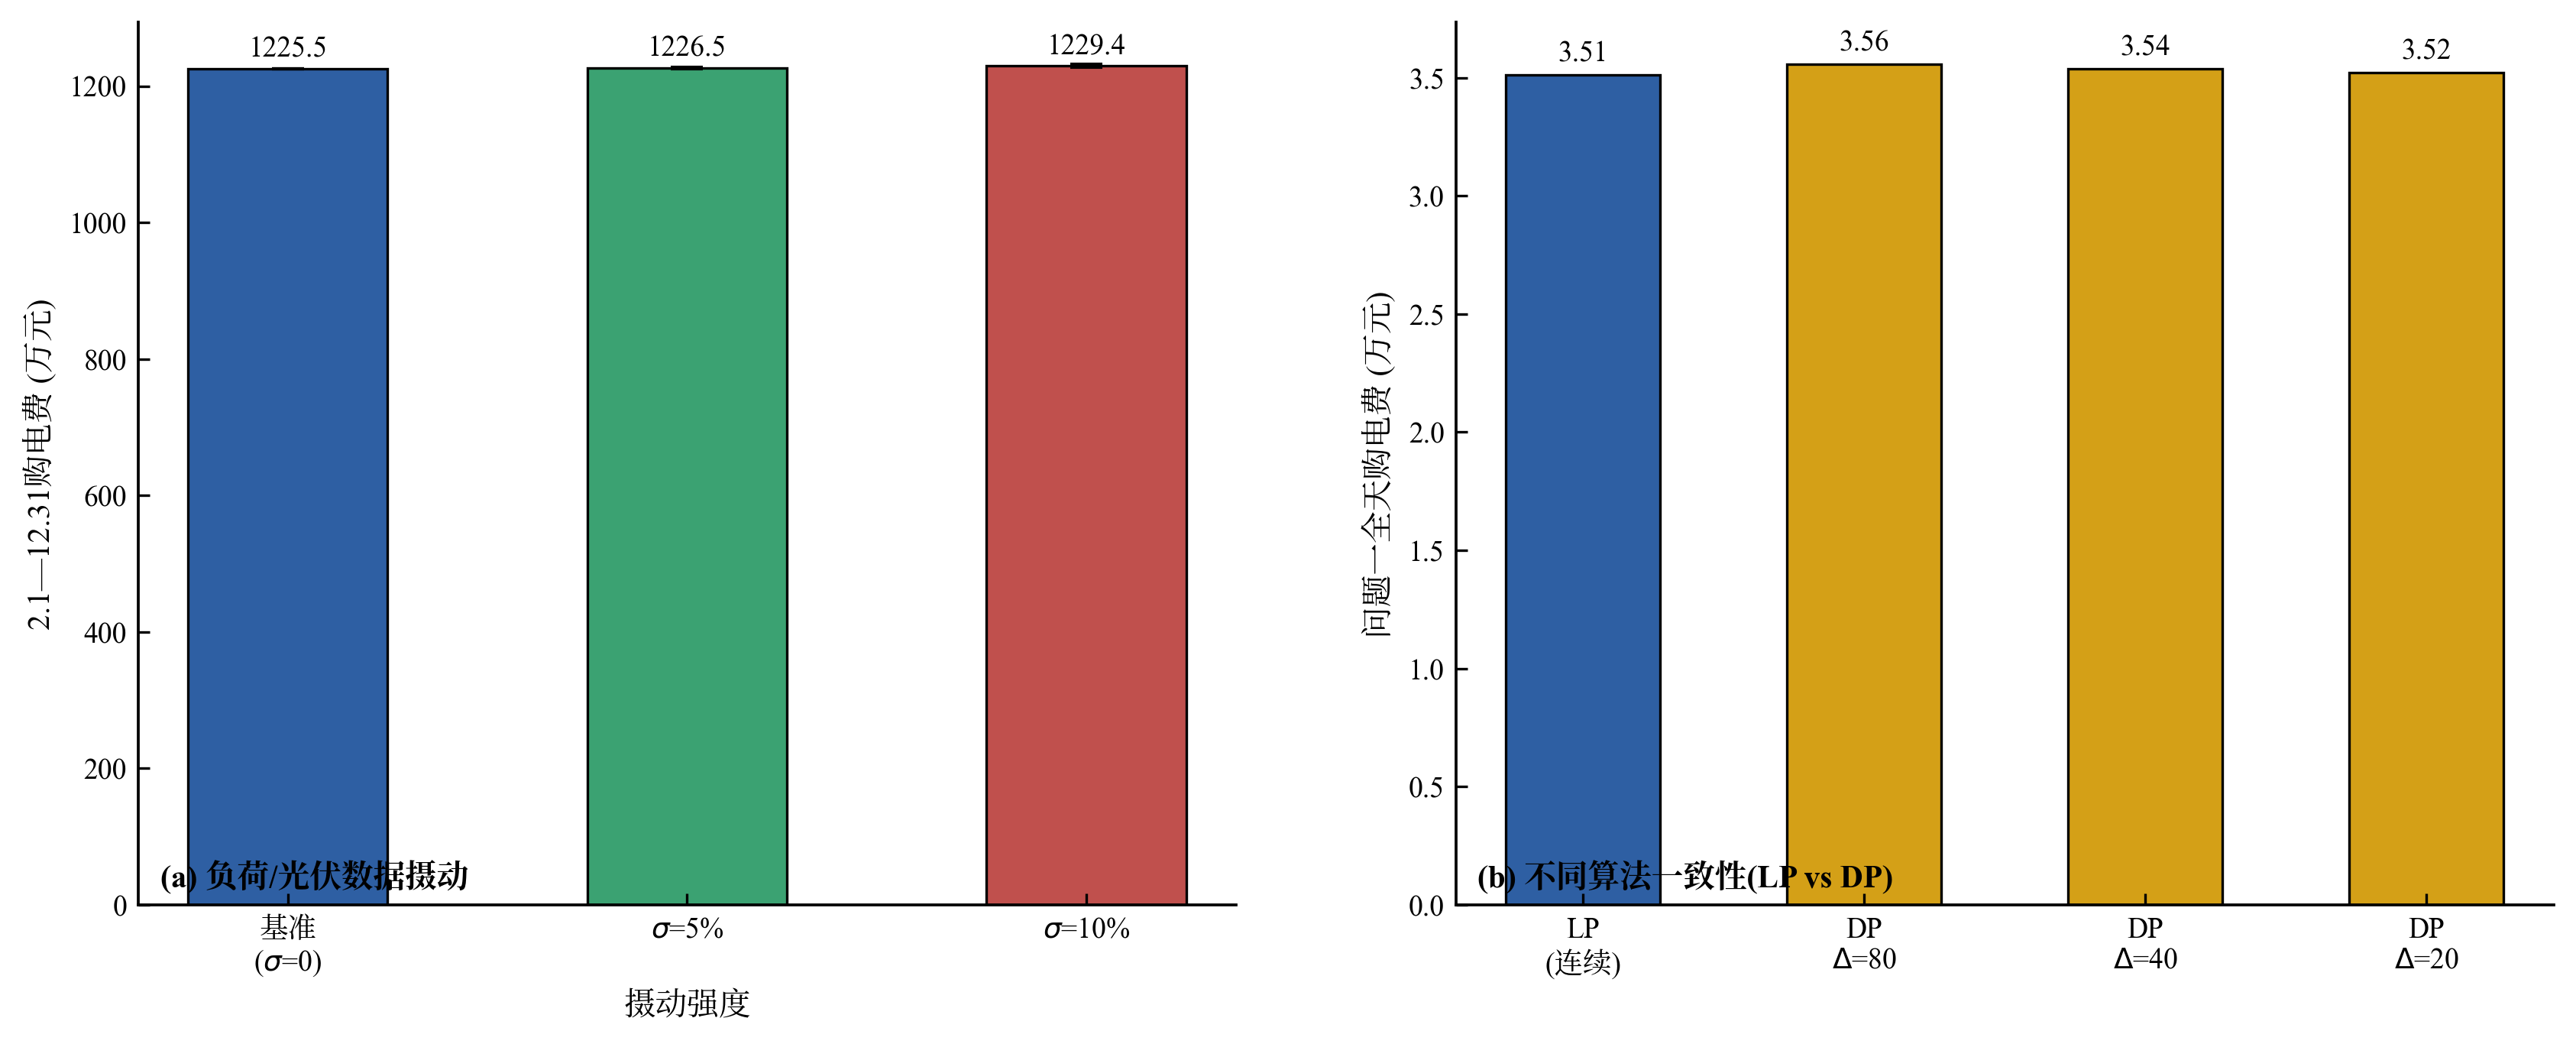
\includegraphics[width=0.88\textwidth]{../求解/图片/图6-1_稳健性检验.png}
    \caption{稳健性检验：数据摄动与算法一致性对比}
    \label{fig:robust}
\end{figure}
